The Modeler allows the user to simply create and edit all processes of the project using the following components:
\begin{itemize}
  \item process editor,
  \item process simulator,
  \item data variable editor,
  \item role editor,
  \item action editor.
\end{itemize}
These components are accessible from the Modeler toolbar by clicking on its icon.
Above the toolbar, there are tabs for each process of the project and a tab with a plus icon which can be used to create a new process.

\subsection{Process editor}\label{subsec:process-editor}

In the process editor component the selected process is displayed.
The upper toolbar contains tools for working with the whole process (import, export, clear, etc.), editing places and transitions (add new, change marking, change label, etc.), editing arcs (create new regular, reset, inhibitor, or read arc, change multiplicity, etc.), and working with the layout (auto align elements, move element, etc.).
Task icons are displayed in the middle of the transition rectangle.

\begin{figure}[h!]
  \centering
  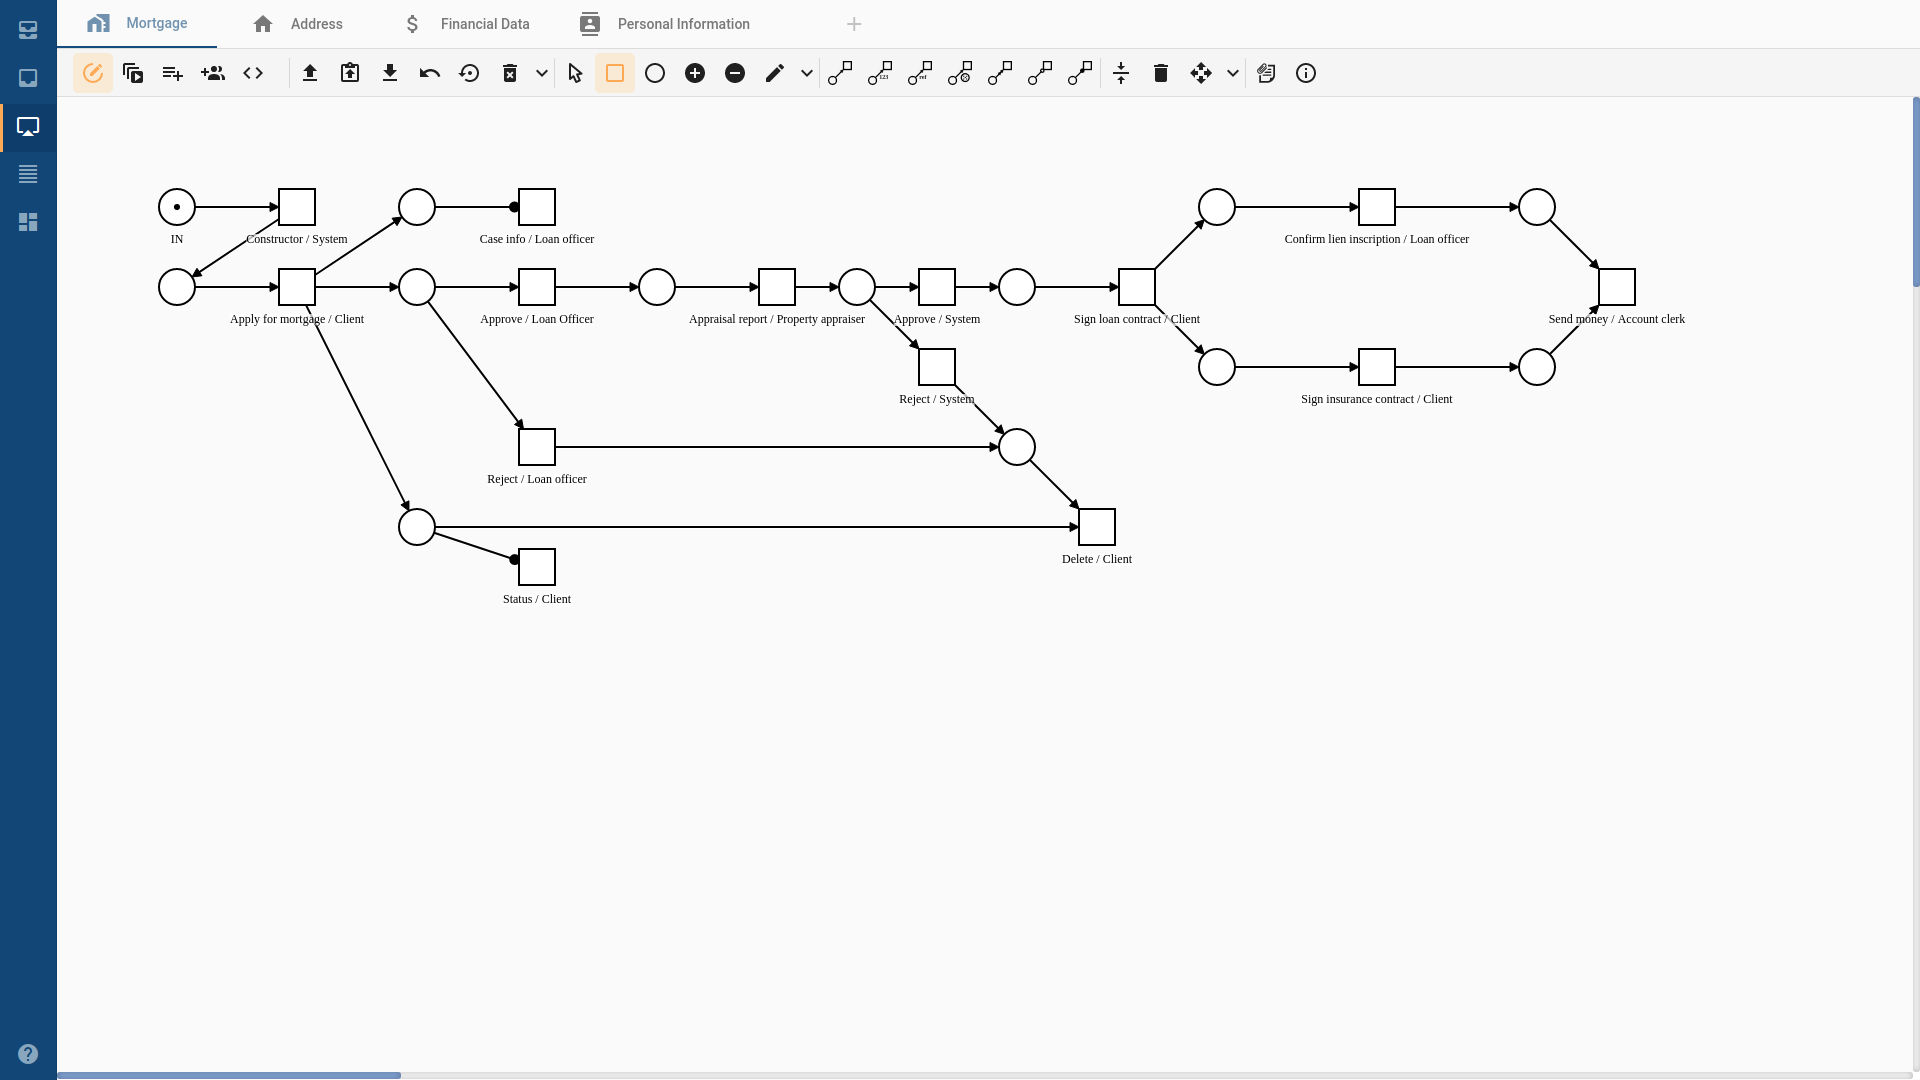
\includegraphics[width=0.9\textwidth]{images/modeler_process_editor.png}
  \caption{Modeler - process editor}
  \label{fig:modeler_process_editor}
\end{figure}

\subsection{Process simulator}\label{subsec:process-simulator}

This view allows users to simulate the execution of a given process (Figure~\ref{fig:modeler_process_simulator}).
There are two modes for different types of simulation - transition mode and task mode.
In both modes enabled tasks are shown with a green border and background.
Inactive tasks are shown with a red border.

In the transition mode clicking on an enabled task will execute it immediately.
Tokens from input places are consumed and new tokens are produced in the output places as defined by the Petri net.

Task mode simulates real execution of the task as it is implemented in the \engine.
Clicking on an enabled task simulates assigning of the given task.
Tokens from input places are consumed and two arrows displayed in the center of the task.
The red arrow cancels the execution, the green arrow will finish the execution and produce new tokens in the output places as defined by the Petri net.

\begin{figure}[h!]
  \centering
  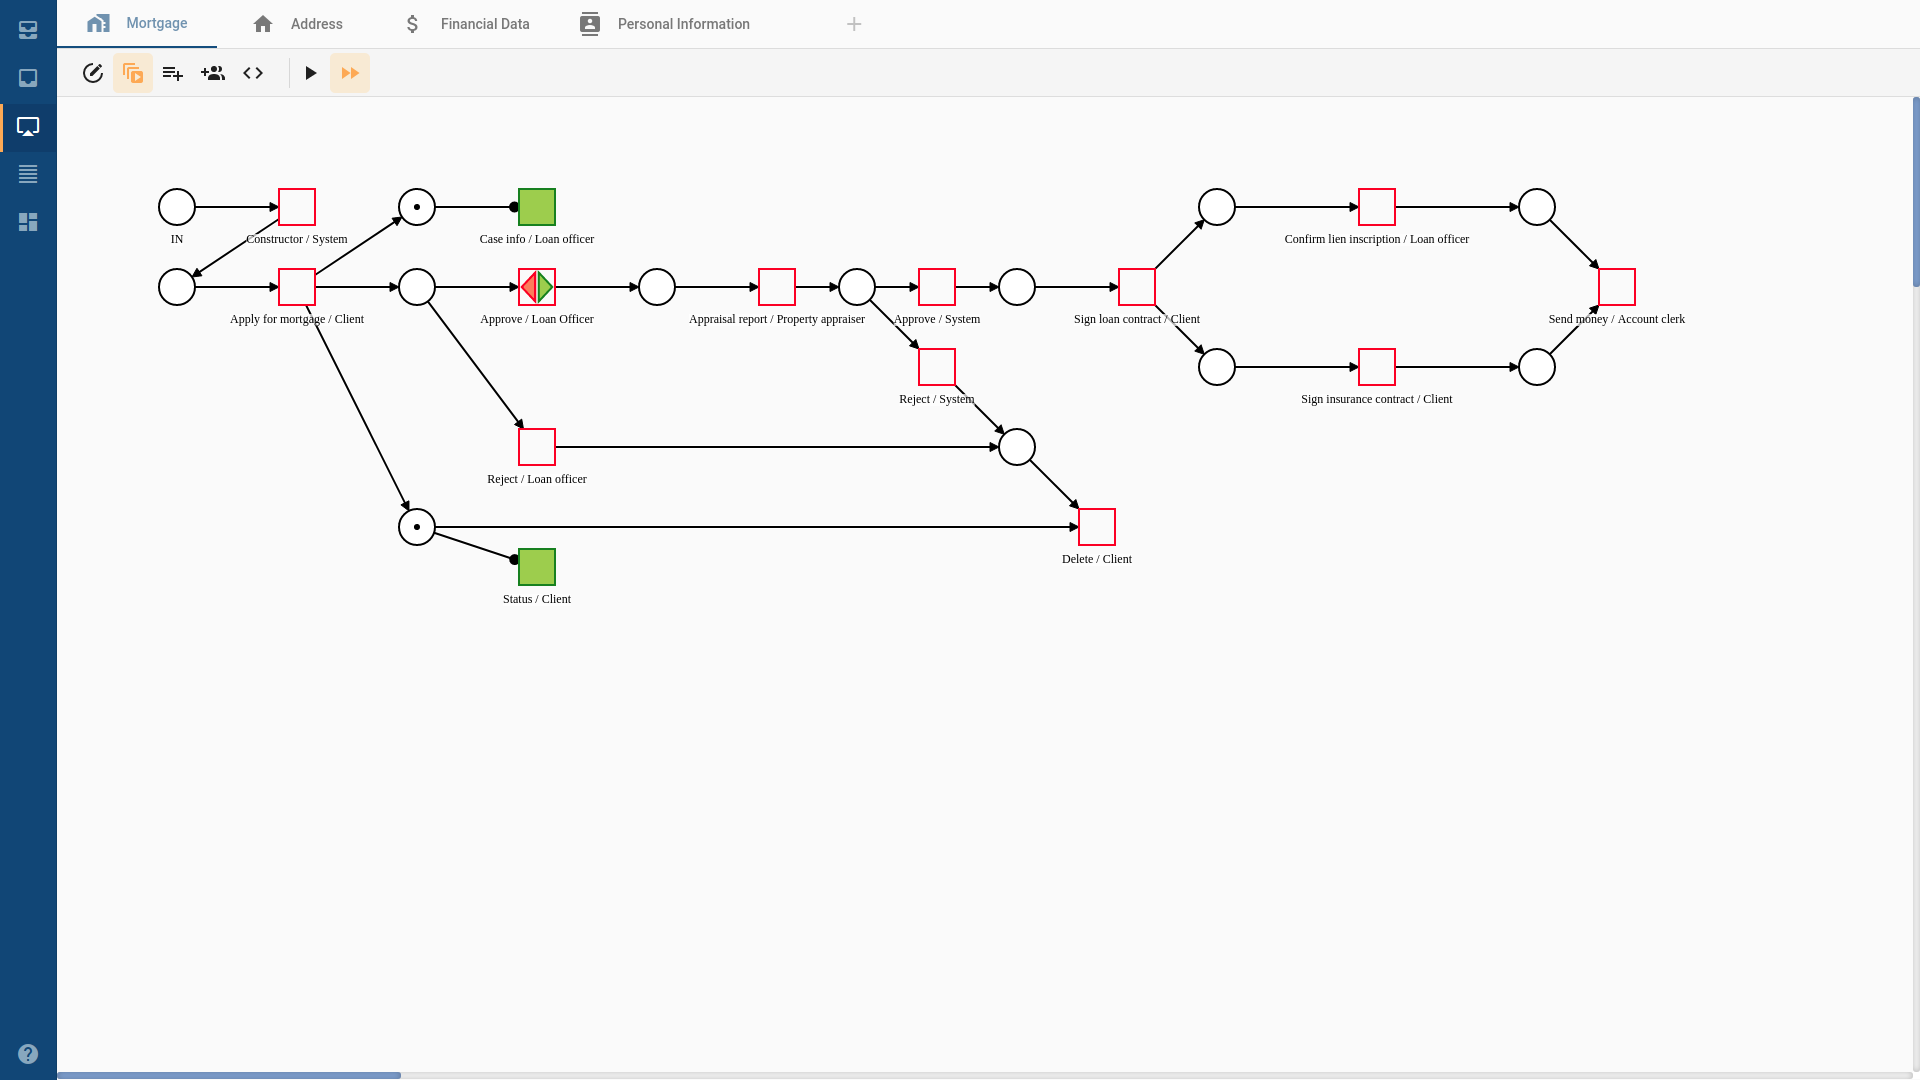
\includegraphics[width=0.9\textwidth]{images/modeler_process_simulator.png}
  \caption{Modeler - process simulator}
  \label{fig:modeler_process_simulator}
\end{figure}

\subsection{Data variable editor}\label{subsec:data-variable-editor}

Data variables are displayed as a master-detail interface (Figure~\ref{fig:modeler_data_editor}).
The master list contains all data variables and allows users to select it by clicking.
The selected data variable is displayed in the detail as an editable form.
All changes are automatically saved.
A data variable can be deleted by clicking the \texttt{Delete data field} button which is displayed while the cursor is above the field's item in the list.

\begin{figure}[h!]
  \centering
  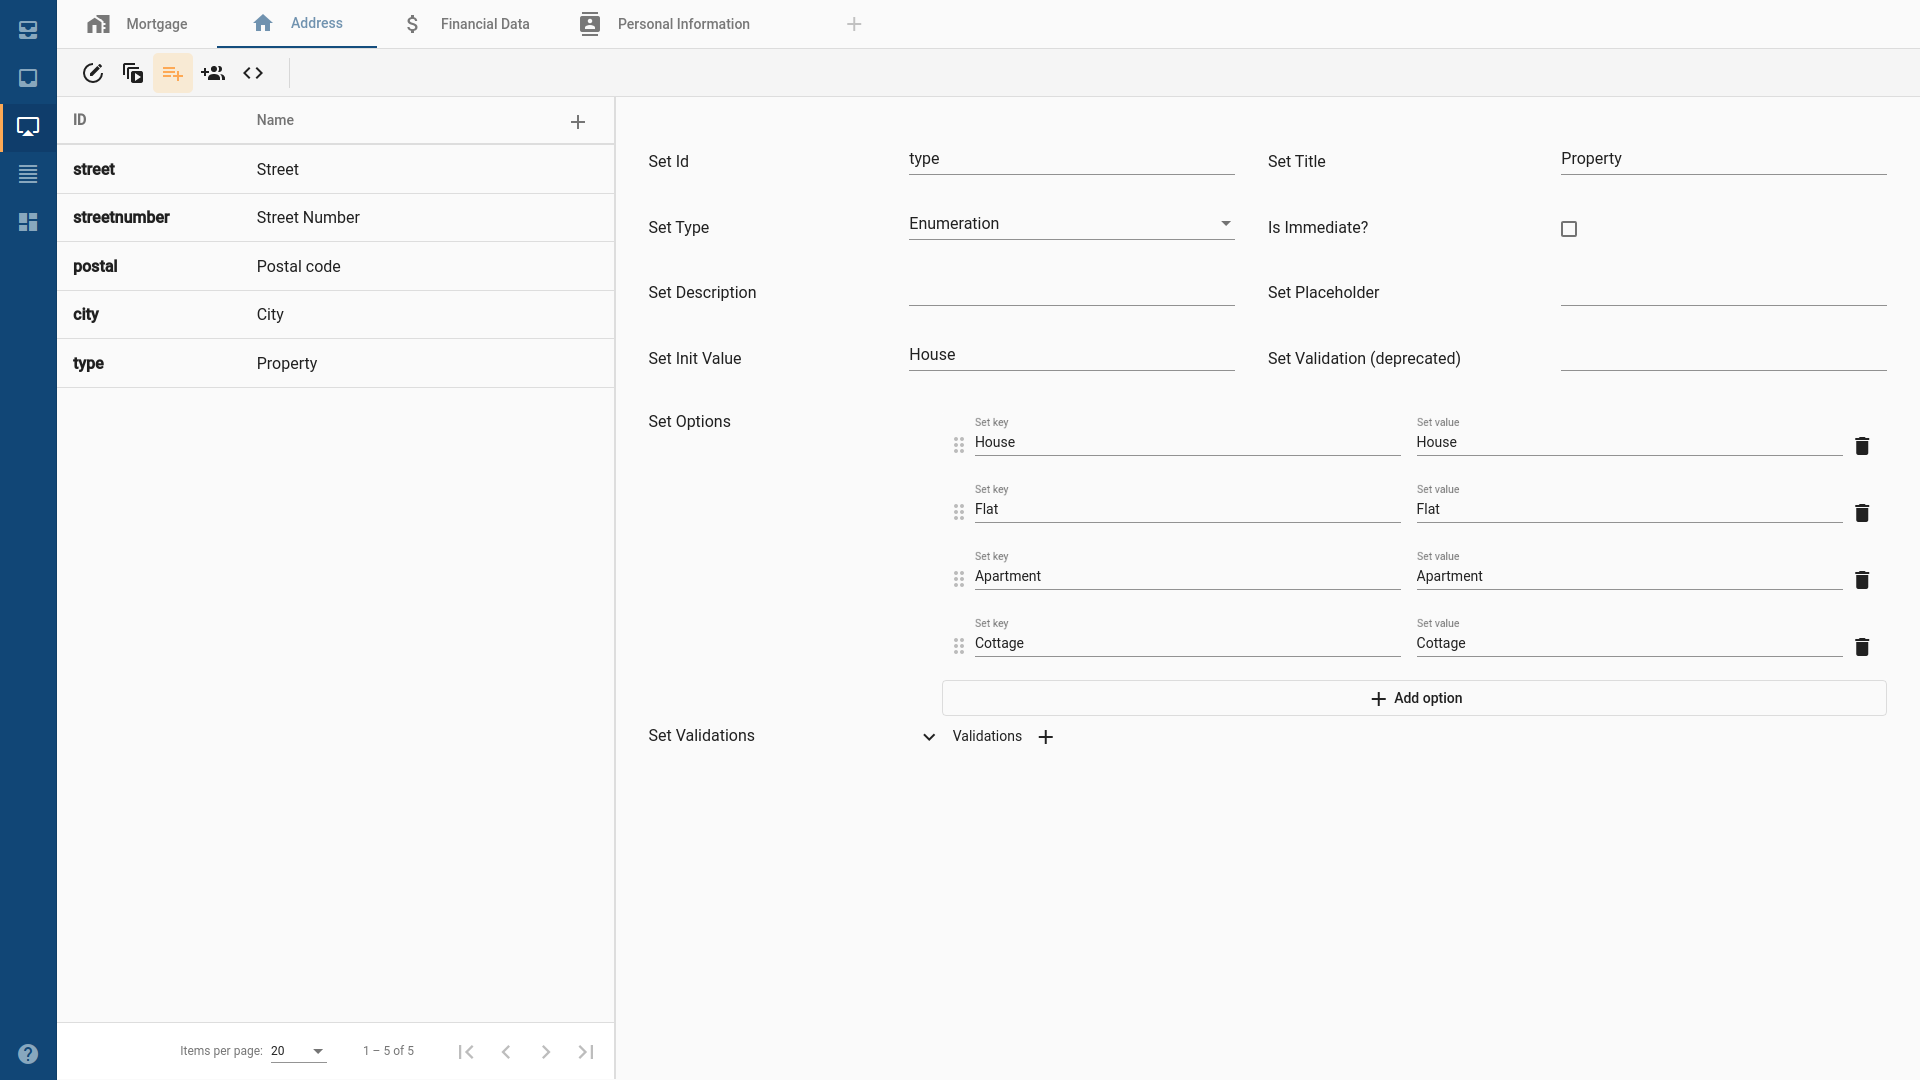
\includegraphics[width=0.9\textwidth]{images/modeler_data_editor.png}
  \caption{Modeler - data variable editor}
  \label{fig:modeler_data_editor}
\end{figure}

\subsection{Role editor}\label{subsec:role-editor}

The Role editor displays all roles of the given process in a pageable list (Figure~\ref{fig:modeler_role_editor}).
Each item shows only id and title, which can be edited after clicking on the list and expanding it into an editable form.
Changes to any field are automatically saved.
Clicking the \texttt{Delete} button at the bottom will permanently remove the role.

\begin{figure}[h!]
  \centering
  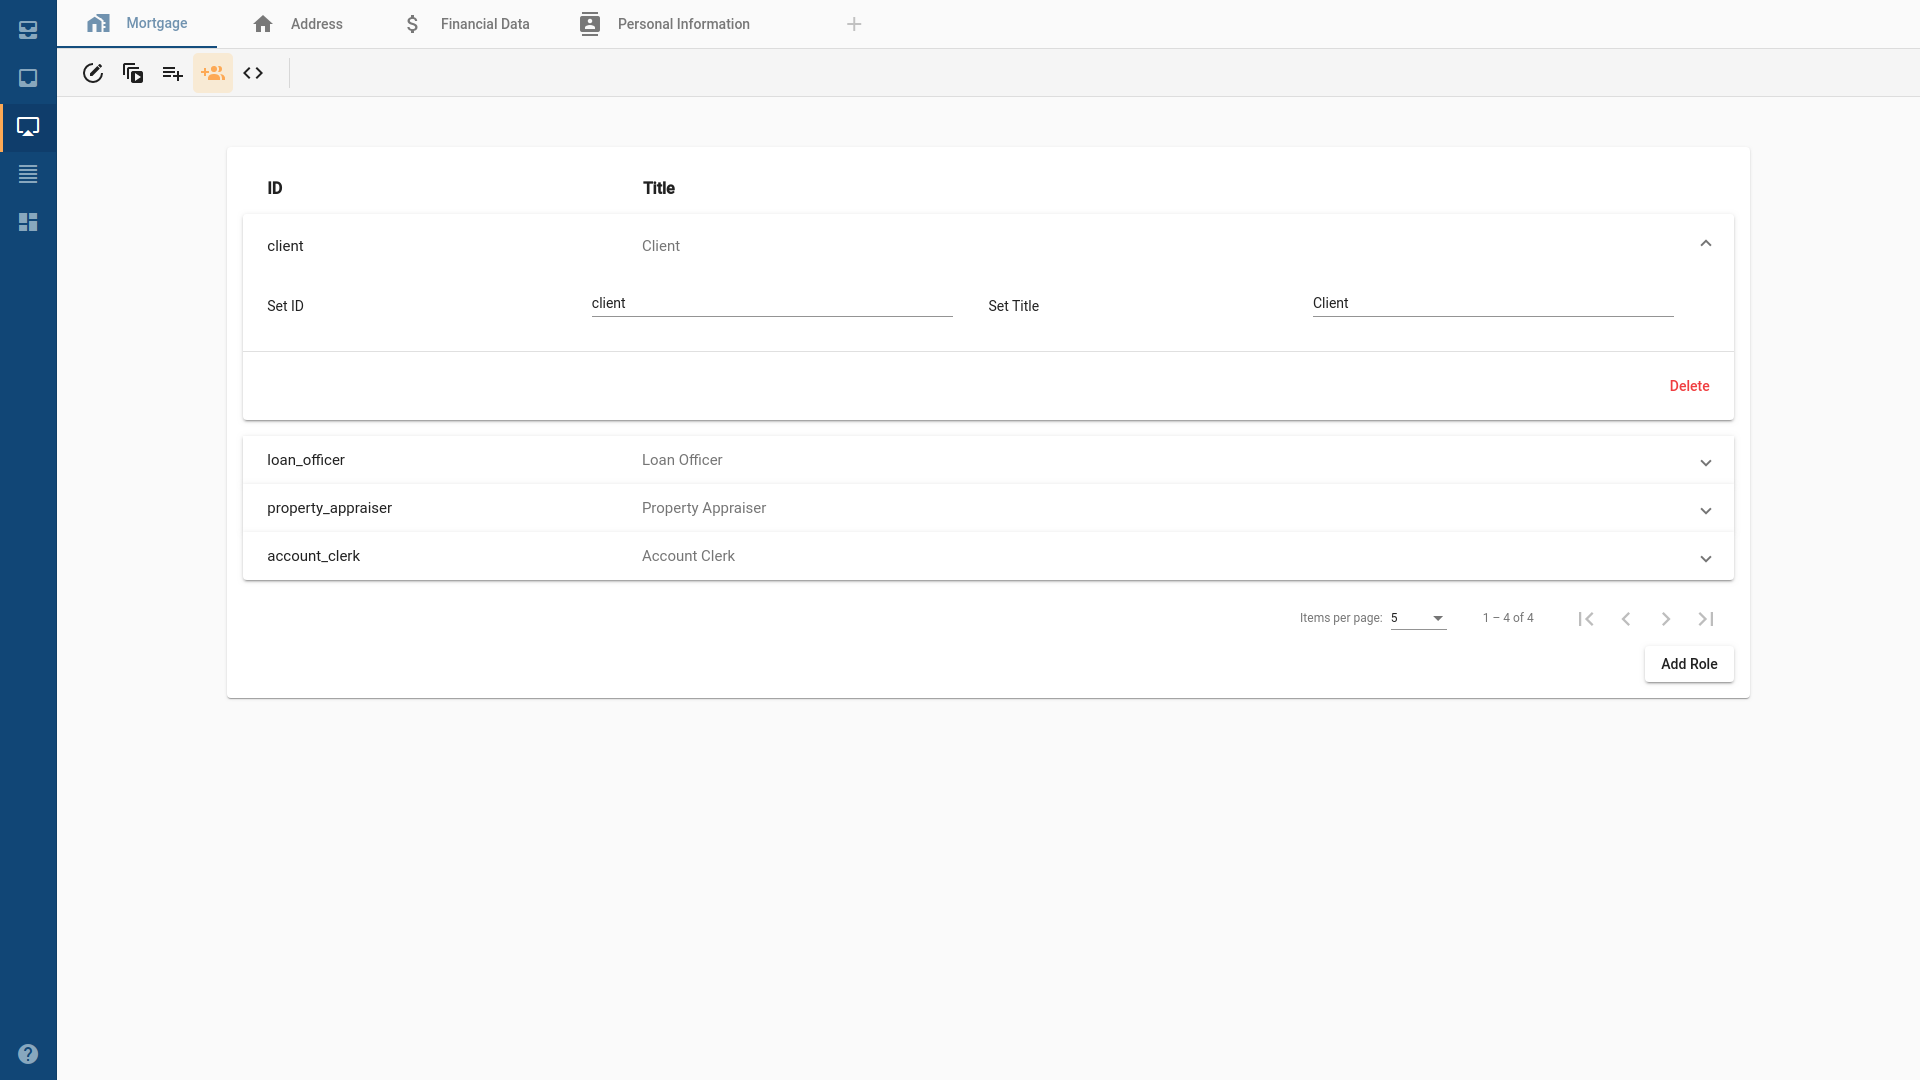
\includegraphics[width=0.9\textwidth]{images/modeler_role_editor.png}
  \caption{Modeler - role editor}
  \label{fig:modeler_role_editor}
\end{figure}

\subsection{Action editor}\label{subsec:action-editor}

The action editor allows users to view, add, and edit actions of the given process as a master-detail interface (Figure~\ref{fig:modeler_action_editor}).
In the editor's toolbar, the user can choose between actions bound to data variables or tasks.

The first option will show a list of all data variables in the master list.
Selecting a data field will show a list of actions categorized by its trigger in the detail.
A new action can be added by clicking on the plus button next to the trigger category.
After expanding the action by clicking on it a code editor is displayed where the user can write the action body.
The code editor shows 10 lines of code by default, but can be resized by dragging the bottom border of the whole action card.

The other option will show a list of all tasks and allows to edit actions bound to events or data fields of the given task.

\begin{figure}[h!]
  \centering
  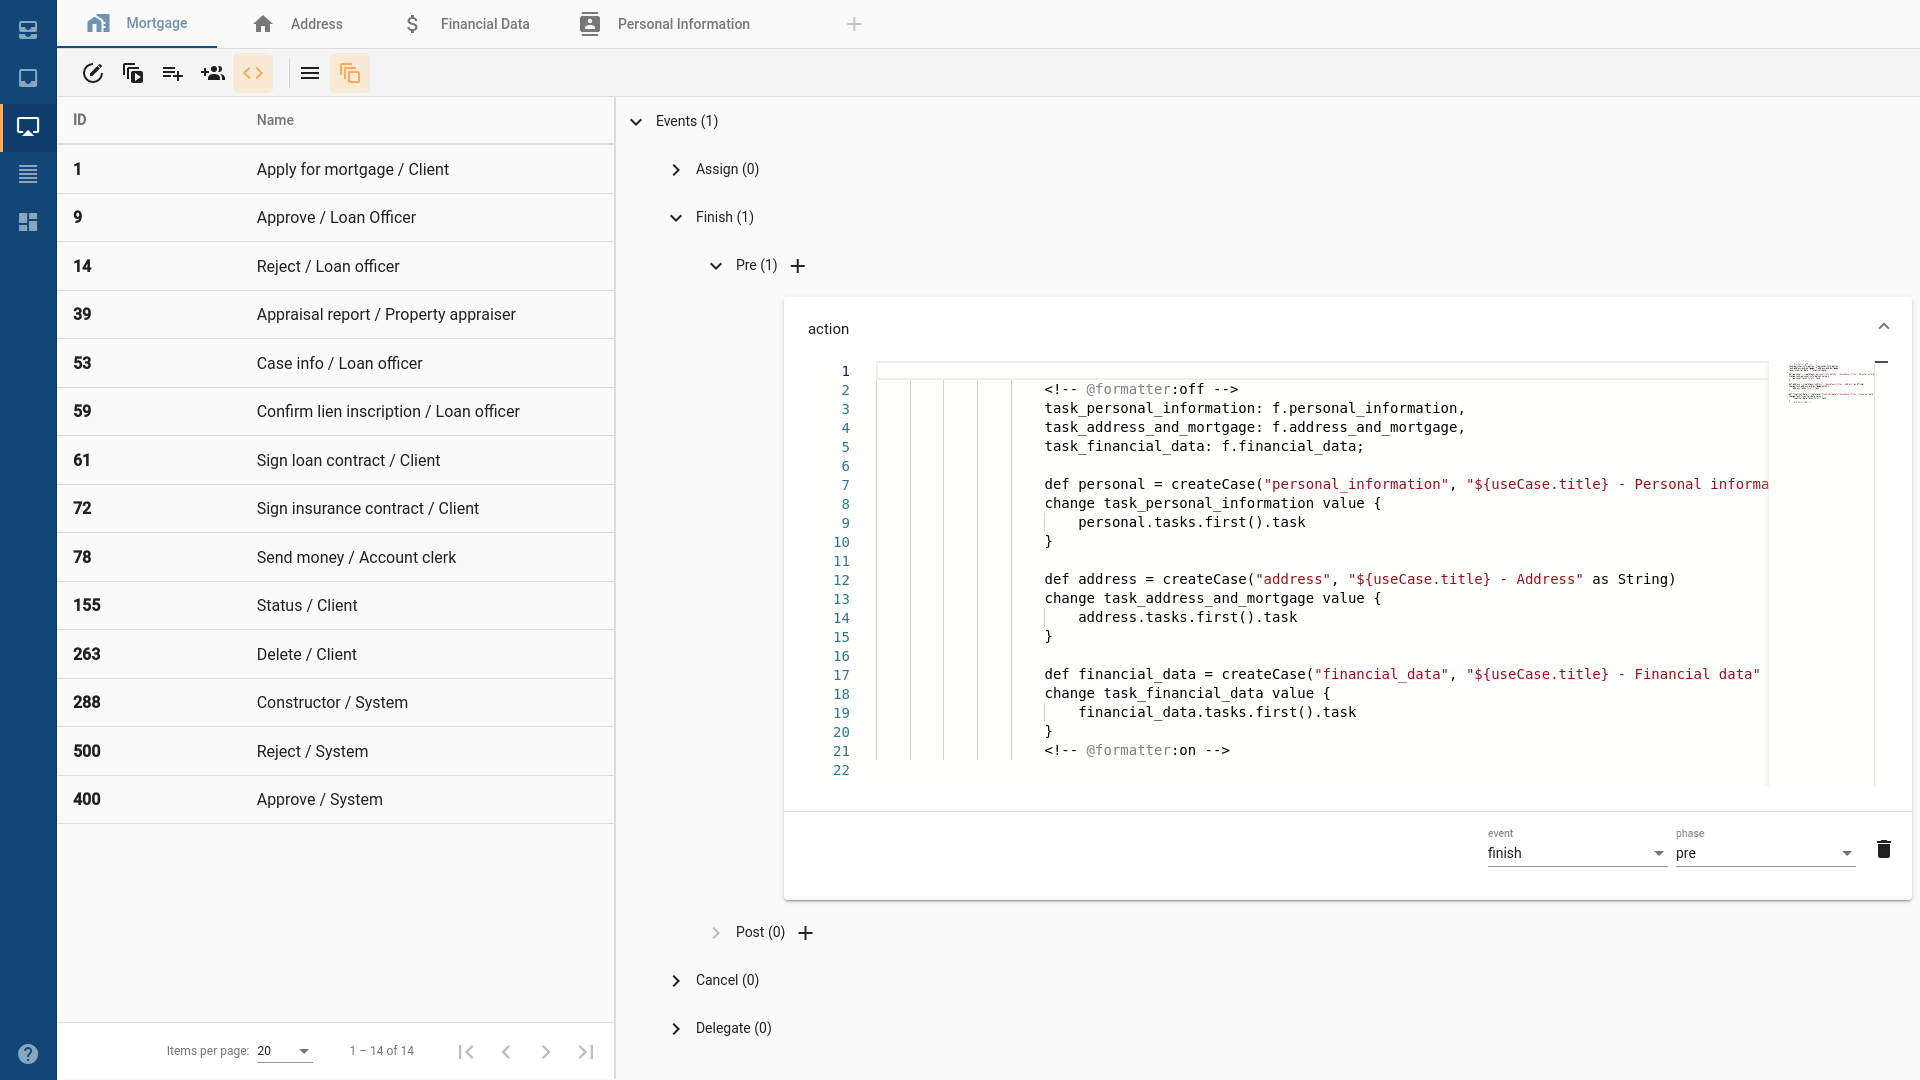
\includegraphics[width=0.9\textwidth]{images/modeler_action_editor.png}
  \caption{Modeler - action editor}
  \label{fig:modeler_action_editor}
\end{figure}
